%%%%%%%%%%%%%%%%%%%%%%%%%%%%%%%%%%%%%%%%%%%%%%%%%%%%%%%%%%%%%%%%%%%%%%%%
%                                                                      %
%     File: Thesis_Introduction.tex                                    %
%     Tex Master: Thesis.tex                                           %
%                                                                      %
%     Author: Israel Sother                                            %
%     Last modified: 27 May 2024                                       %
%                                                                      %
%%%%%%%%%%%%%%%%%%%%%%%%%%%%%%%%%%%%%%%%%%%%%%%%%%%%%%%%%%%%%%%%%%%%%%%%

\chapter{Introduction}\label{chapter:introduction}
\minitoc% Creating a minitoc

%%%%%%%%%%%%%%%%%%%%%%%%%%%%%%%%%%%%%%%%%%%%%%%%%%%%%%%%%%%%%%%%%%%%%%%%
\section{Motivation}\label{section:motivation}
With the increasing regulation efforts to reduce carbon footprints, an upward trend of investments in the mobility sector for the development of electric and hybrid powertrains has emerged. This field has received considerable interest for not only hardware improvements~\cite{Wang:power_converter_review:2020} but also new software alternatives with several new control strategies being proposed. From one side the advancing processing power available in microcontrollers has enabled the use of real-time predictive control strategies~\cite{Karamanakos:MPC_in_power_electronics:2020}, while the use of wide bandgap semiconductors results in a substantial efficiency improvement~\cite{Palmour:wide_bandgap_efficiency:2006}.

Formula Student is an engineering competition that challenges students to design, manufacture, and test a formula-style race car inside a given set of regulations. Similarly to the industry trend, the competition has pushed teams towards electrification, encouraging students to seek solutions that are lightweight, powerful, and efficient. The \gls{fst} was funded in 2001, and since then has built 12 prototypes, from the fourth model (FST04) onward they have an electric powertrain, with the last 3 having autonomous racing mode, with the last one shown in \Cref{fig:fst12_fsg}.

A major advance in the power converter field was the use of wide bandgap semiconductors, which has allowed the development of more efficient converters with a higher power density. As a relatively new technology, there aren't many off-the-shelf solutions that fulfill the specifications required for a Formula Student prototype, thus some of the top teams started to develop their own motor drive solutions\@. \gls{fst} started working on a fully self-developed powertrain in 2017 with the motor development by~\citet{Sarrico:MSc}, and inverter development by Costa~\cite{Costa:MSc}. This development aligns with the fundamental objectives of Formula Student, which is empowering technical and practical knowledge to better prepare students. Additionally, the development of the entire powertrain system can result in a more efficient platform, creating a system optimized for each prototype. Unfortunately, the motor prototype is not ready to be used in the car, and the inverter is missing a system able to control the currently used motors. This work intends to fill a critical gap which is the absence of adequate control for a \gls{pmsm}. By developing and implementing a control strategy that enables the use of an in-house developed inverter with the commercial motor solution, this work not only addresses the identified bottleneck in the powertrain section but also shifts the performance envelope standards, improving the overall capabilities of the next prototypes.

\begin{figure}[!htb]
	\centering
	% \fbox{
		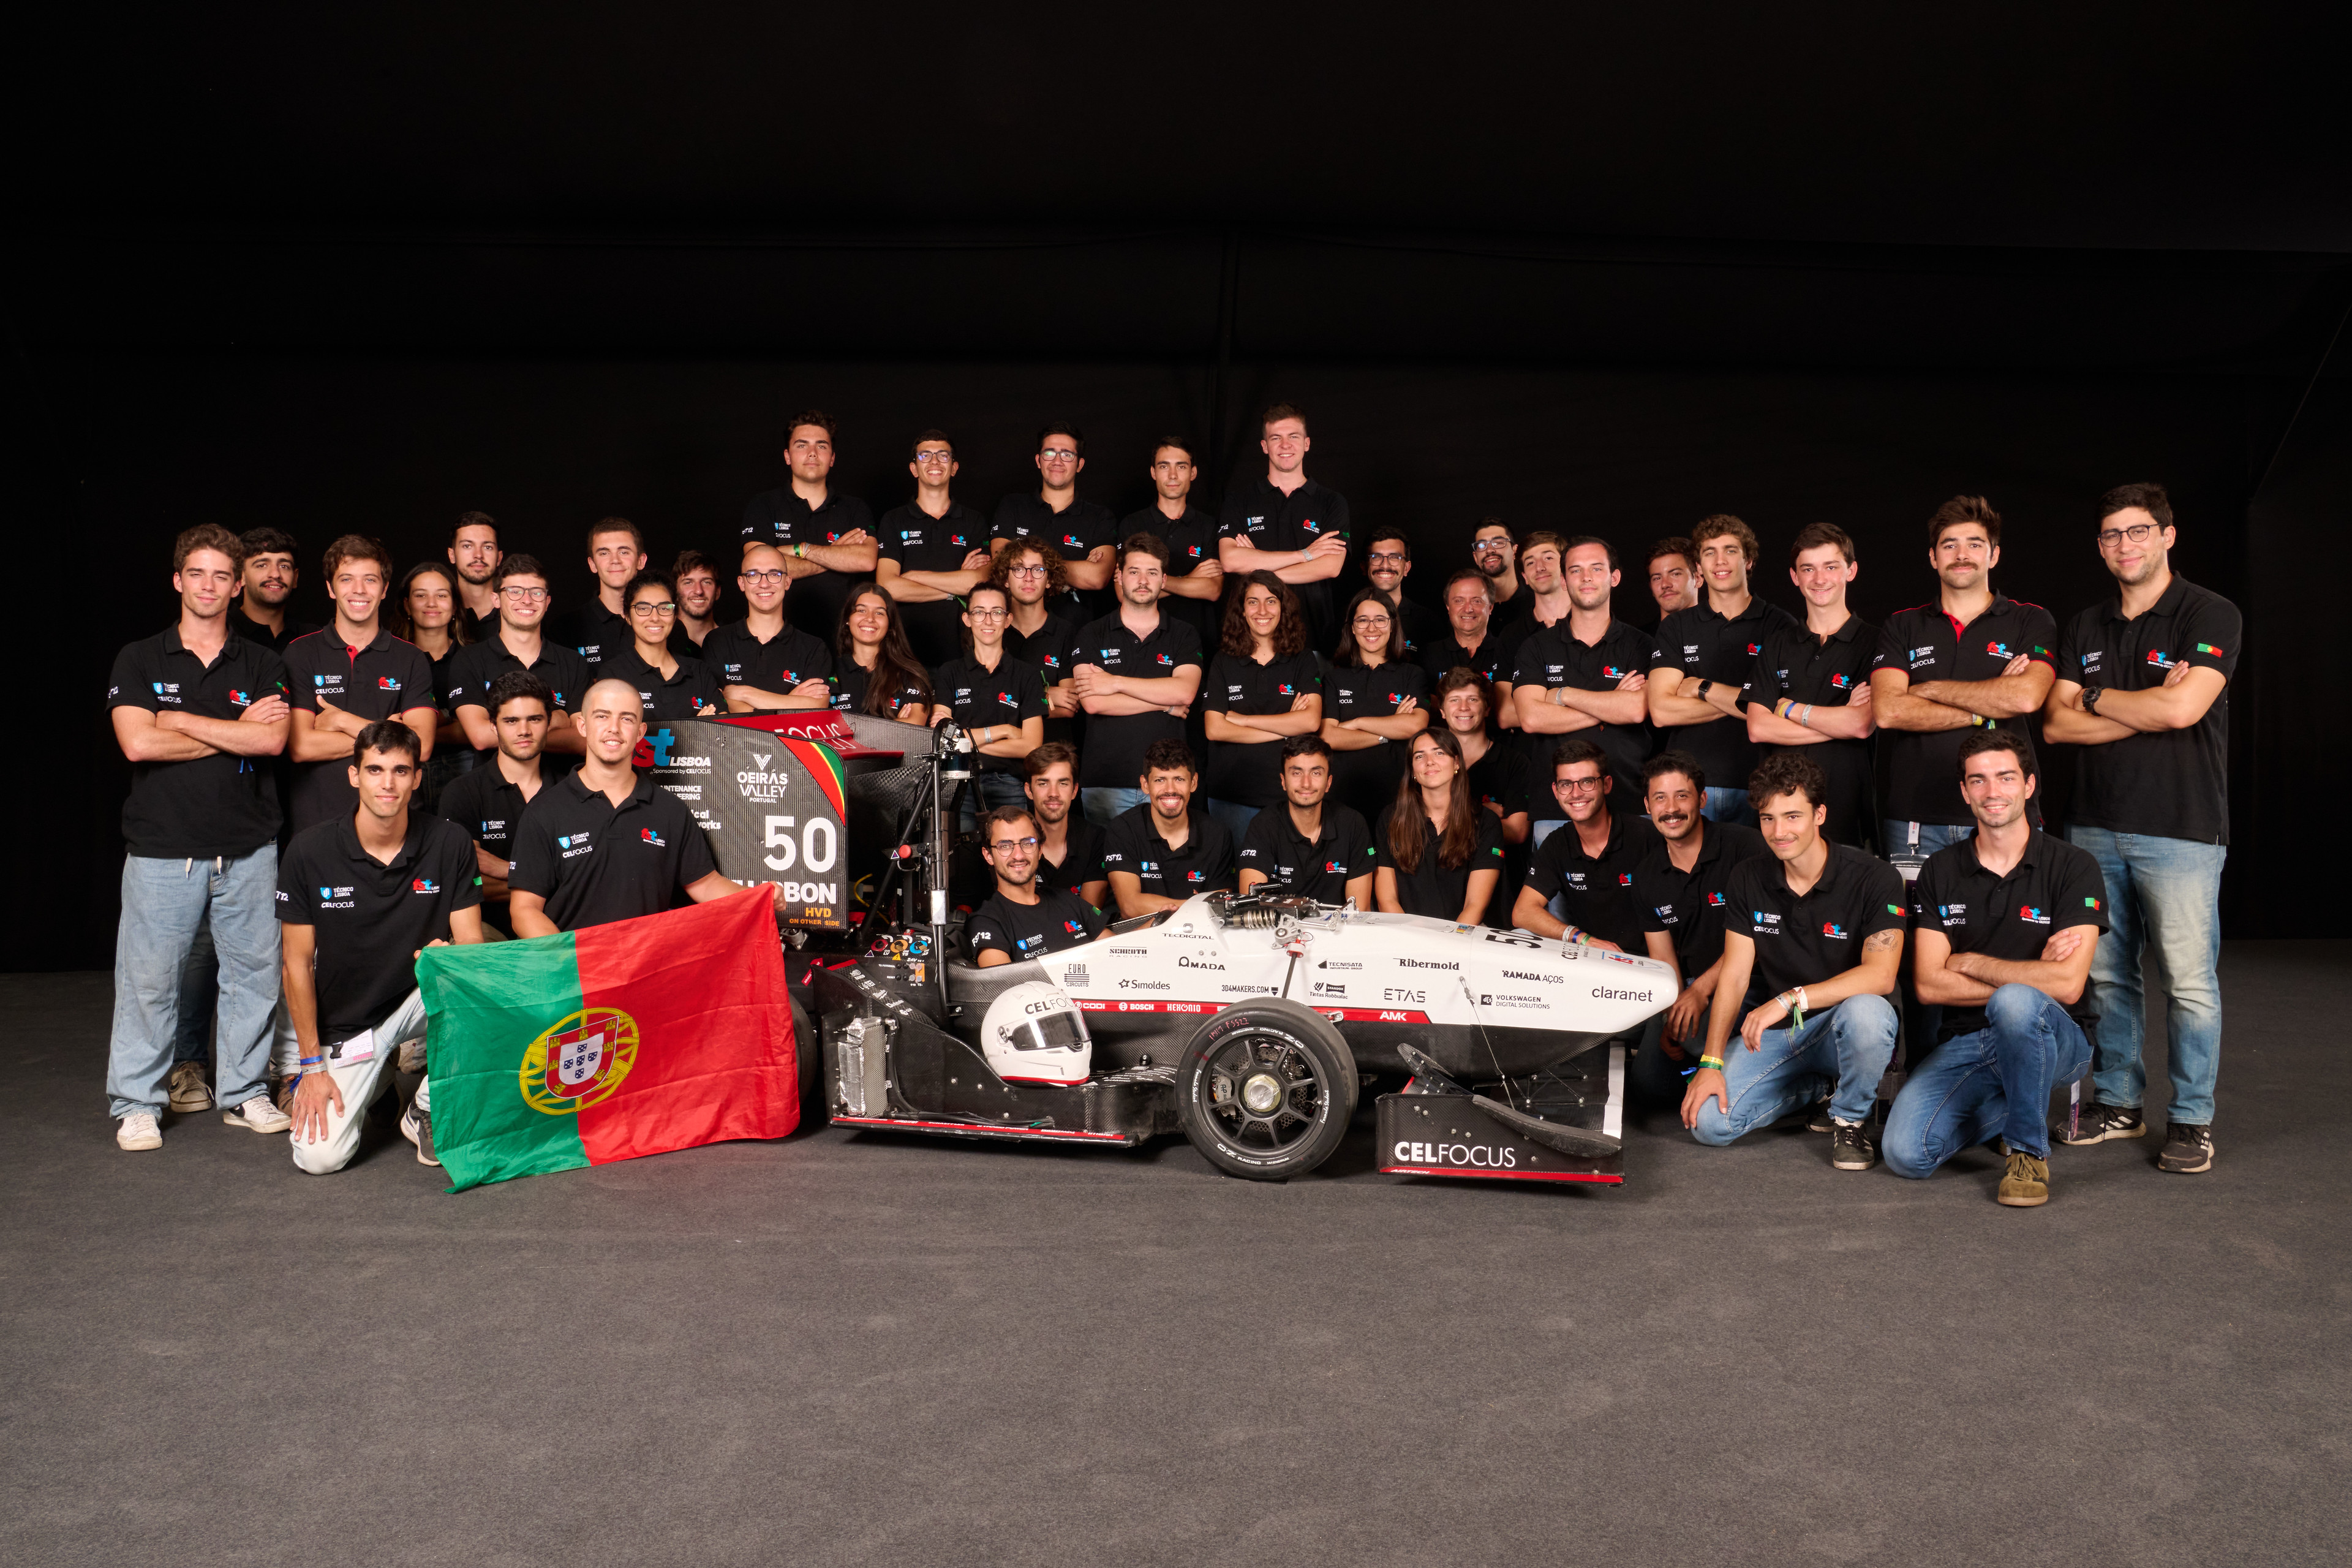
\includegraphics[clip, trim=4cm 18cm 4cm 19cm, width=1\textwidth]{Figures/20230817_11-40-48_7254_grobe.jpg}
	% }
	\caption[FST12 Team at Formula Student Germany Competition.]{FST12 Team at Formula Student Germany Competition, © FSG - Axel Grobe.}
	\label{fig:fst12_fsg}%chktex 24
\end{figure}
%%%%%%%%%%%%%%%%%%%%%%%%%%%%%%%%%%%%%%%%%%%%%%%%%%%%%%%%%%%%%%%%%%%%%%%%
% \section{Topic Overview}\label{section:intro_overview}
\section{Control Methods Overview}\label{section:control_methods_overview}

Through the years, several approaches have been proposed to control synchronous machines using a 2-level three-phase inverter. Regarding the control methods, several solutions have been presented in the literature with the most common being \gls{foc} and \gls{dtc}, with \gls{mpc}~\cite{Bianchi:control_review} being introduced more recently, seeking a compromise between the advantages of \gls{foc} and \gls{dtc}. Some approaches require a modulator such as \gls{svm}~\cite{Neacsu:SVM_intro:2001:IECON}, while others can directly output the semiconductor trigger signals~\cite{Vazquez:MPC_in_power_systems_review:2017:IEEE}.

The use of \gls{foc} and \gls{dtc} have dominated the market for many years due to their simple implementation, but each of them has downsides\@. \gls{foc} combined with current control PID is known for having a slow dynamic response when compared to \gls{dtc}, while in steady-state behavior and disturbance rejection, \gls{foc} shows better results~\cite{Merzoug:FOCvsDTC:2008,Korkmaz:FOCvsDTC:2013,Souad:FOCvsDTC:2008}. \gls{dtc} has a faster dynamic response, with the compromise of a higher torque ripple and a higher current \gls{thd}. \gls{mpc} has been proposed as a combination of the two, exhibiting a good dynamic response while being able to maintain low current and torque ripple. 
% Another advantage of \gls{dtc} strategy is that when using the standard implementation, the control method is based on the stator axis, thus it does not need rotor position sensors (albeit some implementations can benefit from it), thus having a lower cost and a simpler implementation.

Technical advances in the microprocessor industry have allowed the increasing use of \gls{mpc} in power converters and drives~\cite{Vazquez:MPC_in_power_systems_review:2017:IEEE}. This non-linear control scheme provides easy constraint integration while optimizing the control action in real time and is adaptable to different types of electric machines being controlled. The main downside of this strategy is the increased computational cost, which is offset by the decreased cost of computational power.

\gls{mpc} in power systems is usually divided in two categories: \gls{csmpc} and \gls{fsmpc}~\cite{Wang:MPC_in_Electrical_Machines_review:2017:IEEE}, depending on their output signals. The first type calculates the best possible voltage vector and then uses a modulator like \gls{svm} to compose it, while \gls{fsmpc} exploits the fact that a motor drive usually has a limited number of possible voltage combinations and thus predicts the currents for each of those vectors to evaluate the best option. The second approach usually doesn't need a modulator as it only considers the finite set of all possible converter states, although some variations have tried to increase the search space by introducing synthetic vectors that are created from a combination of the native ones. This technique of subdivision and refining vectors can be used to create a quasi-continuous set \gls{mpc}~\cite{Ma:MPC_Syntetic_vector:2014:IEEE}, which, when combined with reducing the search area to the most probable sector, can improve the torque and current ripple without a prohibitive increase in computational cost.
%%%%%%%%%%%%%%%%%%%%%%%%%%%%%%%%%%%%%%%%%%%%%%%%%%%%%%%%%%%%%%%%%%%%%%%%
\section{Thesis Objectives}\label{section:objectives}

This work targets to develop a nonlinear control strategy that allows the use of the existing high-efficiency inverter~\cite{Costa:MSc} with the commercial motors currently used by the team~\cite{amk:DD5-14-10-POW}. This control method must be able to achieve a faster dynamic response than the current inverter used by the team while maintaining or improving the same steady-state performance, and with a sampling time smaller than 20µs to allow a switching frequency of at least 50kHz.

While the improved control method will enhance the performance, not all the gains will come from that, but also the use of an inverter with \gls{sic} mosfets greatly increases the efficiency. The increase in switching frequency shall bring a reduction in the currents \gls{thd} resulting in further efficiency improvements. Lastly, the use of an inverter designed specifically for this motor will reduce the system mass, improving the power-to-weight ratio.

Summing up, this work aims to increase the dynamic response and the efficiency of the powertrain system using wide bandgap semiconductors and nonlinear control methods. This will be verified in simulations, and wherever possible with a prototype in a test bench, where the control method shall be compared with the \gls{oem} system. A revised version of the inverter will also be made, to improve the measurement robustness to \gls{emi} and to increase the maximum current limit of the semiconductors to match the motor's maximum current.


%%%%%%%%%%%%%%%%%%%%%%%%%%%%%%%%%%%%%%%%%%%%%%%%%%%%%%%%%%%%%%%%%%%%%%%%
\section{Thesis Outline}\label{section:outline}

Chapter 2 starts with an overview of formula student competitions, followed by an introduction to two-level inverters. Then a mathematical model for a \gls{pmsm} is developed, laying the ground for the proposal of the control methods The chapter ends with a brief review of the control methods state of the art.

In Chapter 3 the motor characterization methodology is defined and the current reference generation is presented. A load profile that represents the car is also defined, and the controllers studied in this work are proposed.

Chapter 4 presents simulations comparing the control methods and validation of the simulation model with experimental tests.

In Chapter 5 the conclusions are made, analyzing which objectives were fulfilled and proposing topics for future research.